\documentclass[times, 12pt]{article} 
%\usepackage{setspace} 
\usepackage{graphicx}
\usepackage{amsmath} 

\usepackage{url}

\usepackage{epsfig}
\usepackage{listings}
\usepackage{color}

%width:
\setlength{\textwidth}{6.1in}
\setlength{\evensidemargin}{0.7cm}
\setlength{\oddsidemargin}{0.7cm}

%length:
\setlength{\headheight}{0.0in}
\setlength{\textheight}{8.04in}

%%allow more space for figures
%\setcounter{dbltopnumber}{9}
%\renewcommand{\dbltopfraction}{1.0}
%
%
%%special sauce for floating figures:
%\renewcommand{\textfloatsep}{0.2cm}
%\renewcommand{\floatsep}{0.2cm}
%\setcounter{dbltopnumber}{6}
%\setcounter{topnumber}{6}
%\setcounter{bottomnumber}{6}
%\setcounter{totalnumber}{6}
%\renewcommand{\dbltopfraction}{1.0}
%\renewcommand{\topfraction}{1}
%\renewcommand{\textfraction}{0.05}
%\renewcommand{\floatpagefraction}{0.85}
%
\definecolor{dkgreen}{rgb}{0,0.6,0}
\definecolor{gray}{rgb}{0.5,0.5,0.5}
\definecolor{mauve}{rgb}{0.58,0,0.82}

\lstset{frame=tb,
  language=Java,
  aboveskip=3mm,
  belowskip=3mm,
  showstringspaces=false,
  columns=flexible,
  basicstyle={\small\ttfamily},
  numbers=none,
  numberstyle=\tiny\color{gray},
  keywordstyle=\color{blue},
  commentstyle=\color{dkgreen},
  stringstyle=\color{mauve},
  breaklines=true,
  breakatwhitespace=true
  tabsize=3
}



\begin{document}
%\setlength{\topmargin}{-0.2in}


% \title{\bf \large EE/CSCI 451\\ \bf Spring 2016\\ \bf Programming Homework 2 \\ \footnotesize Assigned: February 1, 2016 \\ Due: February 7, 2016, before 11:59 pm, submit via blackboard\\ Total Points: 50}
% \markboth{Journal of \LaTeX\ Class Files,~Vol.~1, No.~8,~August~2002}{Shell \MakeLowercase{\textit{et al.}}: Bare Demo of IEEEtran.cls for Journals}
\title{\bf \large EE/CSCI 451\\ \bf Fall 2019\\ \bf Programming Homework 2 \\ \footnotesize Assigned: September 12, 2019 \\ Due: September 27, 2019, before 11:59 pm, submit via blackboard\\ Total Points: 50}

\date{}

\maketitle

\small

%\vspace{-1.8cm}
\section*{General Instructions}

\begin{itemize}
	\item You may discuss the algorithms. However, the programs have to be written individually.
	\item Submit \textbf{the source code and the report} via \textbf{Blackboard}. The report file should include reports for all problems and should be in pdf format with file name \texttt{report.pdf}. Put all the files in a zip file  with file name \texttt{<firstname>\_<uscid>\_phw<programming homework number>.zip} (do not create an additional folder inside the zip file). For example, \texttt{alice\_123456\_phw1.zip} should contain the source codes, makefile\cite{makefile}, the report and other necessary files.
	\item The executables should be named \texttt{p1} for problem 1 and \texttt{p2} for problem 2. Both \texttt{p1} and \texttt{p2} should only take one parameter, the number of thread. For example, to run the problem 1 with 4 threads, you should enter './p1 4'.
	\item Your program should be written in C or C++. You can use any operating systems and compilers to develope your program. However, we will test your program on a x86 linux with the latest version of g++ and gcc. Make sure you makefile could compile the executables for \textbf{all} the problems (hint: set multiple targets for the makefile) and the name of the executables are correct. If your program has error when we compile or run your program, you will lose at least 50\% of credits. 
\end{itemize}

\section*{Example Program}
print\_msg.c is an example program. You can refer it for thread creation, joining and passing arguments to threads.\\
To compile it, type: gcc -lrt \textbf{-lpthread} -o go print\_msg.c\\
To run it, type: ./go

\section{Parallel Matrix Multiplication [20 points]}
Parallelize the \textbf{naive} matrix multiplication which you implemented in PHW 1 using Pthreads. One simple way to parallelize the algorithm is evenly partitioning and distributing the computation works of the elements of output matrix among the threads and letting the threads work independently in parallel. For example, assuming the matrix size is $n\times n$ and the number of threads is $p$; let thread $\#1$ compute the elements of column $0 \sim \frac{n}{p}-1$ of the output matrix, thread $\#2$ compute the elements of column $\frac{n}{p} \sim \frac{2n}{p}-1$ of the output matrix, and so on. 

\begin{itemize}
\item The matrix initialization is the same as that in PHW 1. The matrix size is $4K \times 4K$. Print out the execution time and the value of $C[100][100]$ in your program.
\item Pass the number of threads $p$ as a command line parameter [1].
\item Report the execution time for $p=1$ (the serial version you did in PHW1)$,4 ,16, 64$ and $256$. Draw a diagram to show the execution time under various $p$. An example diagram is shown in Figure \ref{fig1}. Briefly discuss your observation.
\item In your report, discuss how you partition the computation works of the elements of the output matrix among the threads.
\end{itemize}

\begin{figure}[hbtp]
 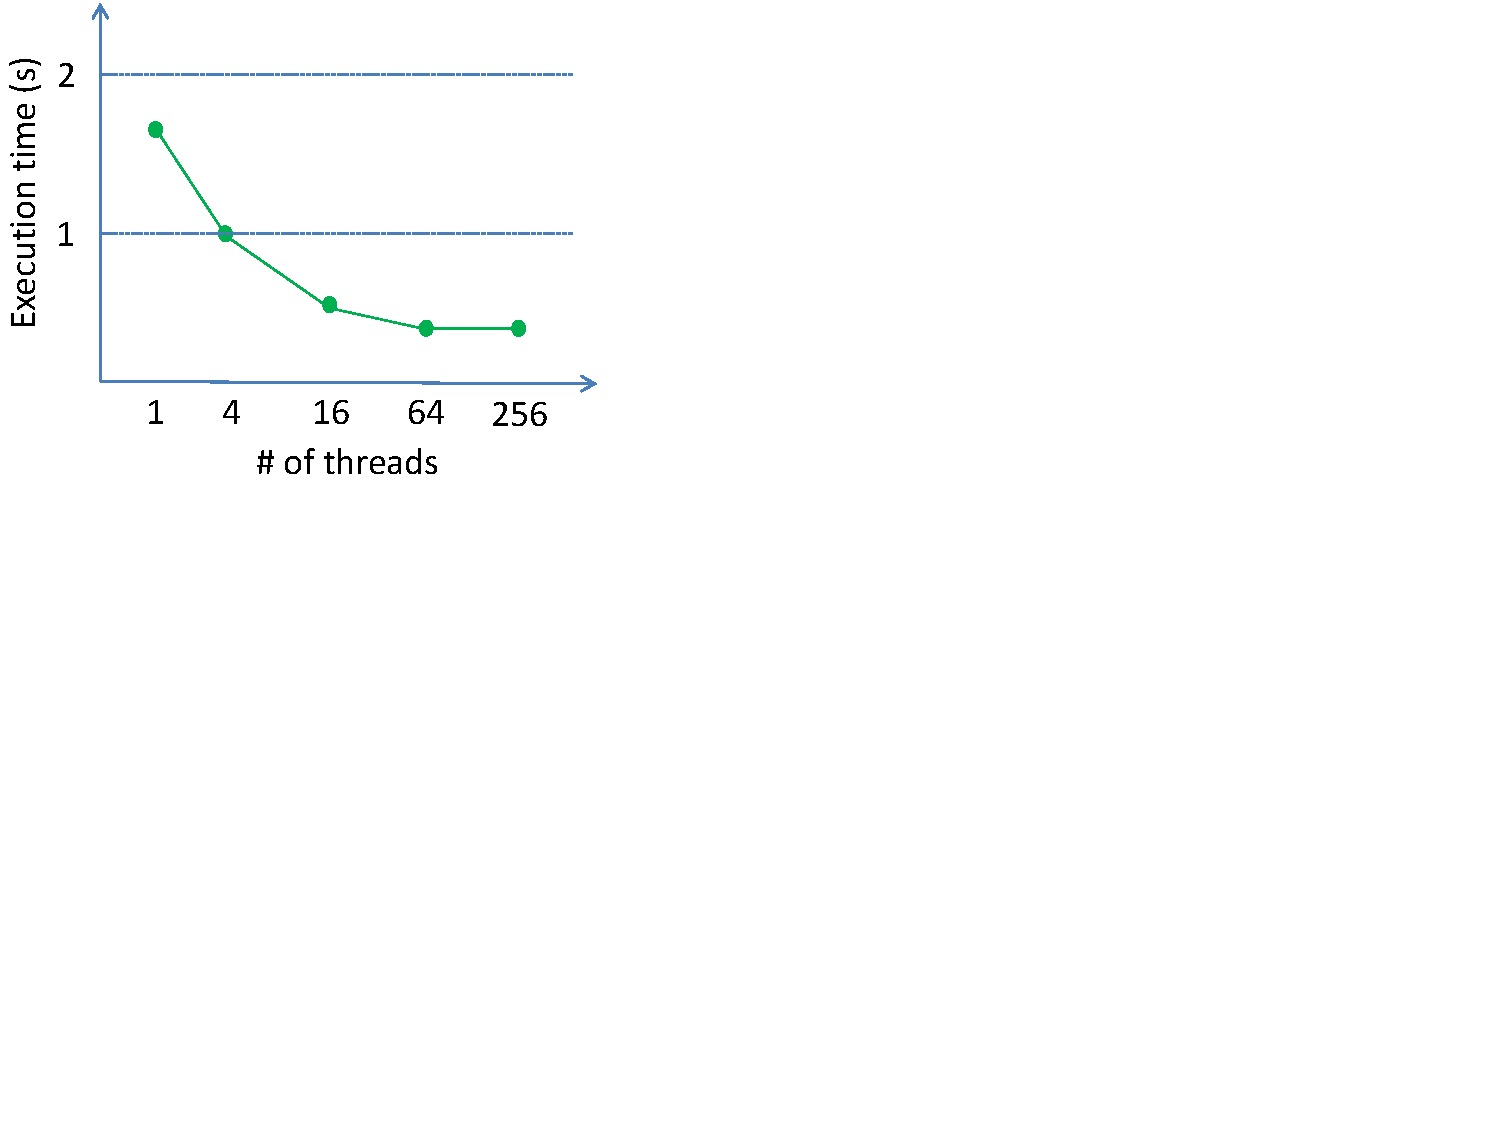
\includegraphics[width=0.45\textwidth,keepaspectratio]{diagram.pdf}
 \centering 
 \caption{Example diagram}	 
 \label{fig1}
\end{figure} 

\vspace{1.8cm}
%\section{Computing $\pi$ [20 points]}
%In Discussion $\#4$, we discussed the algorithm to estimate the value of $\pi$. In this problem, you will need implement this algorithm to estimate the value of $\pi$.
%Let $n$ denote the number of data points you need generate. Let $p$ denote the number of threads.
%
%\begin{itemize}
%\item Serial version [5 points]
%	\begin{itemize}
%			\item $n=1000,000$
%			\item $p=1$ (no need to create thread)
%			\item Print out your estimated $\pi$
%			\item Name the program as p2\_serial.c			
%	\end{itemize}	
%\item Parallel version [15 points]
%	\begin{itemize}
%			\item $n=1000,000$
%			\item $p=5, 10, 50, 100$
%			\item Print out your estimated $\pi$
%			\item Name the program as p2\_parallel.c
%			\item Pass the number of threads $p$ as a command line parameter
%			\item Draw a diagram to show the execution time under various $p$
%			\item Show the speedup compared against the serial version for various $p$
%			\item Briefly discuss your observation  
%	\end{itemize}
%\end{itemize}
%
%To generate a random number between 0 and 1, you may use the rand() function \cite{rand}. For example:
%\begin{lstlisting}
%#include <stdlib.h>     /* srand, rand */
%
%double generate_random_number_between_0_and_1(){
%	return (double)rand()/(double)RAND_MAX;
%}
%
%\end{lstlisting}


\section{Parallel K-Means [30 points]}
In PHW 1, you implemented the $K$-Means algorithm. In this problem, you will need to parallelize your implementation using Pthreads. Let $p$ denote the number of threads you create. The parallel version of $K$-Means algorithm has the following steps:
\begin{enumerate}
\item Initialize a mean value for each cluster.
\item Partition and distribute the data elements among the threads. Each thread is responsible for a subset of data elements.
\item Each thread assigns its data elements to the corresponding cluster. Each thread also locally keeps track of the number of data element assigned to each cluster in current iteration and the corresponding sum value.
\item Synchronize the threads.
\item Recompute the mean value of each cluster. 
\item Check convergence; if the algorithm converges, replace the value of each data with the mean value of the cluster which the data belongs to, then terminate the algorithm; otherwise, go to Step 2. 
\end{enumerate}

In this problem, the input data is the same matrix as in PHW 1 which is stored in the `input.raw'; the value of each matrix element ranges from 0 to 255. Thus, the matrix can be displayed as an image. However, we will have \textbf{6} clusters ($K$=6). The initial mean values for the clusters are 0, 65, 100, 125, 190 and 255, respectively. To simplify the implementation, you do not need check the convergence; run \textbf{50} iterations (Step 2-5) then terminate the algorithm and output the matrix into the file named `output.raw'. 

\begin{itemize}	
\item Implement a serial version without using Pthreads (No need to submit this program).	
\item Implement a parallel version using Pthreads. Name the program as p2.c. Pass the number of threads $p$ as a command line parameter 
\item In your report, you need report the execution time for the \textbf{50} iterations (excluding the read/write time) for $p=4,8$. Compare with the serial version with respect to execution time, discuss your observation. 
\item Show the image of the output matrix in your report. 
You can display the output image, `output.raw', using the imageJ \cite{imageJ} software or the given Matlab script file, `show\_raw.m'. If you use `show\_raw.m', remember to specify the file name in the script. 		
\end{itemize}





% \section{Submission}
% You may discuss the algorithms. However, the programs have to be written individually. Submit the code (p1.c and p2.c) and the report via \textbf{Blackboard}. 
% Your program should be written in C or C++. Make sure your program is runnable. Write clearly how to compile and run your code in the report as well. It is recommended to include a Makefile \cite{makefile} along with your submission. If your program has error when we compile or run your program, you will lose at least 50\% of credits. 

\begin{thebibliography}{1}
\bibitem{command}
``Command Line Parameter Parsing,"\\
\url{http://www.codingunit.com/c-tutorial-command-line-parameter-parsing}


\bibitem{makefile}
``Using make and writing Makefiles,"\\
\url{http://www.cs.swarthmore.edu/~newhall/unixhelp/howto_makefiles.html}

\bibitem{rand}
``rand - C++ Reference"\\
\url{http://www.cplusplus.com/reference/cstdlib/rand/}

\bibitem{imageJ}
``imageJ,"\\
\url{http://rsb.info.nih.gov/ij/download.html}
\end{thebibliography}

\end{document}